 \mysection{The Spriggan}{species-spriggan}

   \flavor{"Is it not enough?" he said in his strange rich magical voice, and pointed across his wide lands with the fingers that summoned wonder. ~\\ ~\\ She sighed: it was not enough. \Tilde Lord Dunsany} 

  \mysubsection{Appearance}{spriggan-appearance}
  
  You hail from Elfland, beyond the reach of the Hound of Sish.  Like your brothers and sisters the Myrkálfar you are the Nomadic People, the Rom - cursed with curiosity and infected with the fire that burns in the hearts of the Hallowed to know more, to see the passage of time, and to breathe the air of decay.  All it cost was your soul.  

  You cannot find your way home again, for the bright line between this world and Elfland ebbs forever before you.  Wherever you are is where Elfland cannot be.

  Your bloodline allows you to strike bargains with the lowest of the Small Gods, the Forgotten who stand at the threshold of the Void.  The fear of oblivion dominates every desire and scheme of these sanguinary spirits.  You steal them away from the doorway of Nothingness and by Remembering them, allow them to touch reality once again.  In Remembering, you allow their souls to mingle inside of you, and sing through you - so that in the never-ending ache of Acheron you might, for a moment, remember the feel of the heat of Elfin hearths and the smell of the lavender fields you dream of.  

  You are tall, lithe, and ethereal; Spriggan often stand over 2m, with leaf-shaped ears, long fingers, and gaunt faces vaguely reminiscent of deer or goats.  Older Spriggan often appear cadaverous - while you can't die from old age, your body begins to rot outside of the realm of Elfland (this has no effect on your powers).  Your skin and eye color is as varied as the Mortal races, and from a distance you might pass for human - except for the horns.  Some are small, barely noticeable stubs while other Spriggan sprout deer antlers, curling ram's horns, or tree branches.  It is not uncommon for birds to roost on your horns if they are well developed enough 

    \begin{center}
      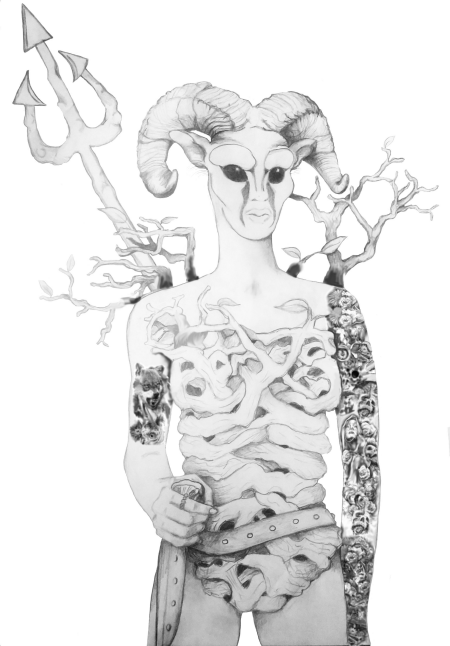
\includegraphics[scale=.5]{Spriggan_Pencil}
    \end{center}


  \mysubsection{The Basics}{spriggan-basics}

  \myhighlight{Supple}{spriggan-flesh}

   Spriggan have a d6 \FLESH
   

  \myhighlight{Uncanny Sight}{spriggan-uncanny-sight}

  You add your \LVL to any \RO or \RB attempt that includes your Awareness.  The \UD still moves \DCDOWN on a natural 1 or 2.

  Your uncanny sight also means you cannot be Surprised (including the Drop), and you can see hidden and invisible creatures.

  \newpage

  \mysubsection{Creation}{spriggan-creation}

  \callout{
    \mynumlist {
      \item Start one of the core Skills at \mybold{Trained (d8+1)}
      \item Start one of your Saves at \mybold{Preserved (d8+1)}
      \item Move your Awareness \DCUP (it should now be a d8)
      \item Write down your Virtues, Complications, and Starting Gear
    }
  }

  \mysubsection{Virtues}{spriggan-virtues}

  \myhighlight{Remembrance of Elfland}{spriggan-virtues-remembrance-elfland}

  Though you have been cast out of Elfland, the noble blood of the King of Elfland still runs through your veins.  You may use this sanguine supremacy to summon and command \mylink{the Abandoned}{forgotten-abandoned} and the \mylink{the Obliterated}{forgotten-obliterated} (collectively known as  \mylink{the Forgotten}{arcana-forgotten}), ghosts who live at the edge of oblivion.

The Abandoned are Small Gods whose names have disappeared from the tongues of men; they exist only as a line in a book buried by the sands of the deserts, etched on forgotten stela in the wilderness, or scribed on scrimshaw lost beneath the waves.  When an Abandoned's name is finally lost, they become the Obliterated - totems and symbols of what they once were, raw power in the form of beasts (through the \mylink{Anamnesis of the Beasts}{forgotten-anamnesis-beasts}), elementals (through the \mylink{Anamnesis of the Elements}{forgotten-anamnesis-elements}), and devils (through the \mylink{Anamnesis of the Damned}{forgotten-anamnesis-damned}).

Three aspects allow you to control the Forgotten:  \mybold{Remembrance}, \mybold{Sovereignty}, and \mybold{Potential}.  You begin with a Remembrance, Sovereignty, and Potential of 1 each
    

  \myhighlight{Anamnesis of the Beasts}{spriggan-virtues-anamnesis-beasts}

   You can summon and control the Obliterated Beasts - mundane animals and Zoological Monsters.  See the section \mylink{Anamnesis of the Beasts}{forgotten-anamnesis-beasts} in Arcana.

  \myhighlight{The Hound of Sish}{spriggan-virtues-hound-of-sish}
  
  You are untouched by Time, the last remnants of godhood.  You are immune to aging, and your \DEATH starts at \mybold{Tough} (d12)  

  \myhighlight{Tongues of the Forgotten}{spriggan-virtues-tongues}

  You know how to speak Archaic, Fiendish, and Seraphic in addition to any other languages you might know.

  \mysubsection{Complications}{spriggan-complications}

  \myhighlight{Antlers}{spriggan-complication-antlers}

  Antlers or tree branches grow from your head; birds often roost there (and if they do, you can speak with them).  You can't wear helmets or use a Bow or Strongbow. You can't attack with your antlers, but you can sacrifice them for the same effect as wearing a helmet. Antlers will regrow during a Vacation.


  \myhighlight{Iron allergy}{spriggan-complication-iron-allergy}

  You are allergic to iron.  If you touch iron it will deal 1 Flesh damage to you every Moment.  Iron weapons do an extra 2 points of damage if they strike Flesh

  \myhighlight{Unhallowed}{spriggan-complication-unhallowed}
    
  You have no "soul" and are Unhallowed. You can't enter consecrated ground and are affected by the Mystic ability "Curse the Unhallowed"


  \mysubsection{Starting Gear}{spriggan-starting-gear}

  \mybullet {
    \item a pair of workgloves;
    \item two silver daggers and a spear; 
    \item a set of prayer candles;
    \item a block of salt (for licking) and a pouch of dead mice;
    \item a pouch of 3 gems (roll on the \mylink{Gems table}{appendixb-random-treasure} in Appendix B);
  }
